\chapter{Online Optimzation of Nonlinear Dynamics Experiments}
This chapter presents the results of the experiments carried out during the this masters project. There are two set of important results: i) experiments carried out in late 2022 and ii) experiments carried out in the first semester of 2023. In the first batch of experiments, the experimental method and setup was still being perfected. We attempted optimzation using the kick resilience as objective function and learned it was not the best choice. We moved on to using instead the Injection Efficiency as objective, which had a better performance.  In ii), we continued using the injection efficiency. We started to take more care when choosing the knobs, avoiding the families close to their magnatic nonlinear regime and experimenting with different possibilities of constraints. We also carried out optimzation in different working tunes and had the time to perform further characterization and analysis of the found configurations.
\section{Kick resilience optimization attempt}
\label{experiments22}
In the first attempt to online otpimze the nonlinear dynamics, we used the beam kick resilience as objective function. As mentioned in section, we sought to minimize the beam-loss rate at a given fixed dipolar kick. The idea was to minize for a given kick, increase the kick and repeat the process, reaching higher kicks resilience.
\subsection{The knobs}
The knobs were chosen according to the compensation scheme described in section: the achromatic families SDA0, SDB0, SDP0, SFA0, SFB0, SFP0, and the chromatic families SDA1, SDB1, SDP1, SDA3, SDB3, SDP3, SFA1, SFB1, SFP1 varied freely. The SDA2, SDB2, SDP2 and SFA2, SFB2, SFP2 families were the compensation families used keep chromaticity constant when varying the optimization knobs.
\subsection{Objective function and setup}
Before firing the experiment, a small beam current was accumulated into the storage ring, usually $10~\unit{mA}$, localized in a single bunch. At a given moment, we can fire up the kick from a dipole kicker, located close to the injection section. The BPMs acquisition was fired in synchrony with the kick. Since we are interested in optimizing the horiontal DA, the kick is in the horizontal direction. The scheme below sketches the $x,x^\prime$ phase space during the experiment. For small kicks, in the linear approximation, the beam would receive an anction-jump along the $x^\prime$ axis and start to rotate along the corresponding ellipse. In the nonlinear regime, the ellipses are distorted, but we expect the same overall behaviour: action jump along the angles which is eventually translated into horizontal oscillations. Thus, the larger the kick resilience, larger the DA.
\todo[inline]{move the phase-space discussion to the previous chapter as well as figure illustrating it}
To evaluate the beam loss we used the BPMs sum signal, which is proportional to the stored current. The average sum-signal of the first 10 turns was compared to that of the last 10 turns in a X turns BPMs acquisition. The kick strength was chosen to render an initial beam rate loss of about 35\% up to 60\%
\subsection{Optimization runs \& results}
With the aforementioned scheme for changing strengths in the sextupole families, RCDS was started to minimize the beam-loss upon the horizontal kick. In the algorithm's first iteration\footnote{An RCDS iteration is reached upon completing the one-dimensional optimization along all directions in the parameter space. After each iteration, the algorithm constructs a new (conjugate) direction according to Powell's method and may replace existing directions by this new conjugate direction.}, beam loss dropped from 60\% to nearly 0\%. In the beginning of the 2nd iteration, the objective function took negative values, which is a numerical artifact, so the optimization run was stopped. The beam-loss minimization significantly improved the beam's resiliency to dipole kicks. After the optimization, it was necessary to kick the beam at approximately $\Delta x^\prime=-0.850~\unit{m rad}$ to achieve the same  30--60\% beam-loss rate previously achieved by a $\Delta x^\prime=-0.760~\unit{m rad}$ kick.

By the end of this first attempt, the machine magnets were standardized\footnote{Standardizing magnets cosnsists on driving their power suplies with decaying sinusoidal waveforms to remove hysteresis effects and bring the magnets yokes to their standard reference magnetization.} and the configurations found during optimization were loaded into the machine sextupoles. This was done to test the repeatability of the configuration found. Given the improvements in the resilience, it was expected the injection efficiency would also improve as a result of the DA enlargement, however, when trying to inject in the off-axis scheme, the efficiency was quite low, indicating no DA improvements in the $-x$ direction at all. The improved kick resilience, however, was preserved. This observation raised the suspicion that the aperture along the negative horizontal direction might have been negatively impacted by the procedure, while the aperture along $x^\prime$ increased. In other words, the optimization was not evenly distributed along both $x$ and $x^\prime$. The DA border apparently is way more elastic than anticipated, and apparently can be stretched preferentially along $x$ or $x^\prime$, as the Figure X illustrates. This observation motivated the adoption of injection efficiency to probe the DA.
% \begin{figure}
    % \begin{minipage}{0.48\textwidth}
    %     \centering
    % 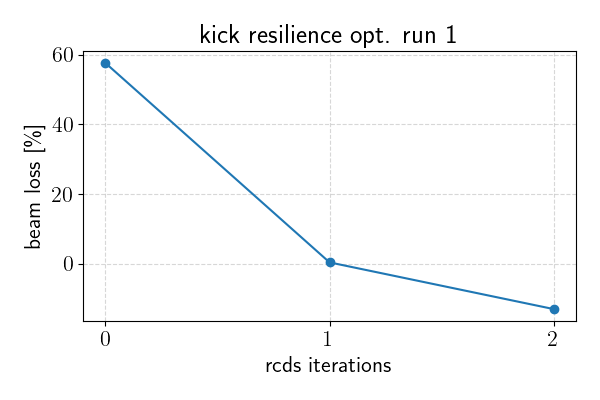
\includegraphics[width=\columnwidth]{Images/beam_loss_hist_run1.png}
    % \caption{Objective function history vs. iterations of the first trial at beam-loss optimization.}
    % \label{beam_loss_hist}
    % \end{minipage}
%     \hfill
%     \begin{minipage}{0.48\textwidth}
%         \centering
%         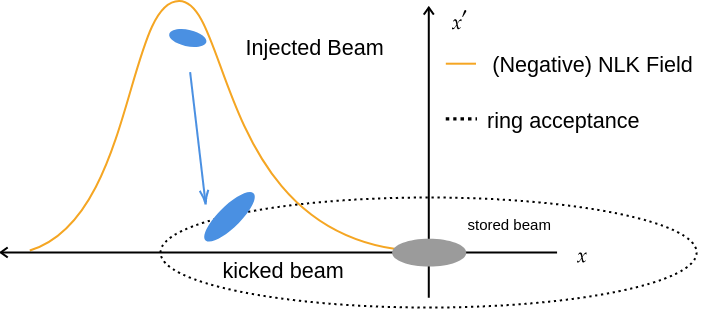
\includegraphics[width=\columnwidth]{Images/inj_cond.png}
%         \caption{Injection conditions for DA optimization}
%         \label{fig:inj_cond}
%     \end{minipage}
% \end{figure}
\missingfigure{illustrate the suspicion about the DA stretching}
% \begin{figure*}[t]
%     \centering
%     \includegraphics*[width=\textwidth]{beam_loss_sexts.png}
%     \caption{Sextupole families strengths and strength changes before/after the beam-loss rate optimization}
%     \label{beam_loss_sexts}
% \end{figure*}

% \subsection{Injection efficiency optimization - december 2022}
% The first attempt at optimizing DA by minizing beam-loss revealed that the optimization procedure did not improve injection efficiency. We started another attempt, using the injection efficiency itself as objective function. The knobs (parameter space) used were the same as in the beam-loss optimization.
% \begin{itemize}
%         \item Objective function \& setup:\\
%         The off-axis injection efficiency was worsened by reducing the NLK strength
%         %$-2.45~\unit{m rad}$ to $-2.25~\unit{m rad}$
%         so the beam was injected in the upper-left border of the  $(x,x^\prime)$ aperture (see Figure~\ref{fig:inj_cond}). The efficiency under such conditions was about 30\%. The maximization of injection efficiency under such injection conditions should correspond to a maximization of the DA evenly among the $x$ and $x^{\prime}$ directions, as opposed to the increase on the $x^\prime$ direction only, as seemed to be the case in the previous attempt.
%         \item Experiment:\\
%         In the first run, within three iterations the injection efficiency reached 70\%,  as shown by Fig.~\ref{injeff_hist1}. The algorithm stopped as it reached the maximum number of the objective function evaluations. A second run was launched, starting from the sextupole configurations just found in the first ruun. In four iterations, 85\% efficiency was reached, as Fig.~\ref{injeff_hist2} shows.
%         \item Results:\\
%         When the NLK strength was restored to the reference value, meaning the nominal off-axis injection conditions were restored (in which the beam ``lands"~ not at the border but within the acceptance), the injection efficiency fluctuated around 95--100\% with good repeatability. There was a severe reduction in beam lifetime by the end of the last optimization trial. Measurement indicated 54.12 hrs lifetime at $15~\unit{mA}$ current, while, the reference (non-optimized) configuration, lifetime at this same current is about 68 hrs.
%     \end{itemize}
% \begin{figure}
%     \begin{minipage}{0.49\textwidth}
%             \centering
%             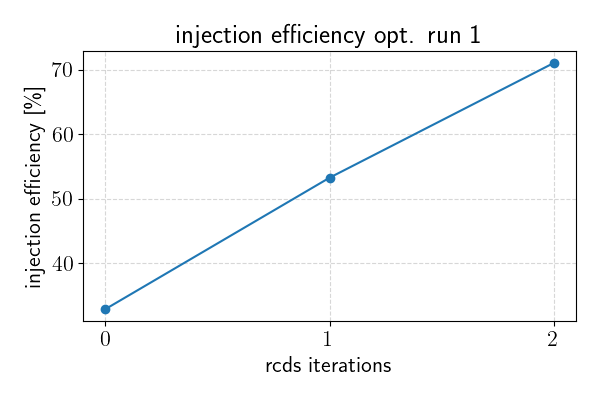
\includegraphics[width=\textwidth]{Images/injeff_hist_run1.png}
%             \caption{Objective function vs iterations during the first run of injection efficiency optimization}
%             \label{injeff_hist1}
%     \end{minipage}
%     \hfill
%     \begin{minipage}{0.49\textwidth}
%             \centering
%             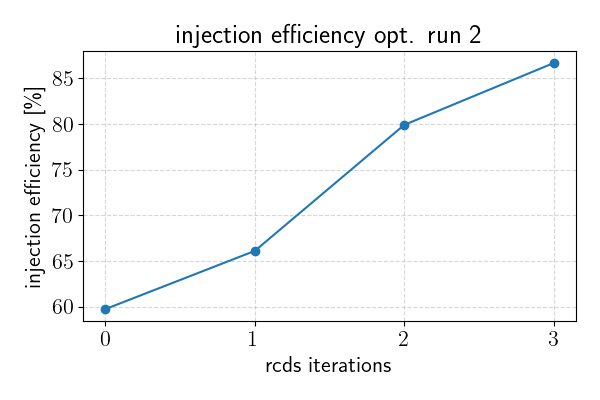
\includegraphics[width=\textwidth]{Images/injeff_hist_run2.png}
%             \caption{Objective function vs iterations during the second run of injection efficiency optimization}
%             \label{injeff_hist2}
%         \end{minipage}
% \end{figure}

% We carried out chromaticity measurements in the machine loaded with the reference configuration (ref-config) and with the sextupole configurations found at iterations 0, 2, and 3 of the last injection efficiency optimization run
% (run shown by Fig.~\ref{injeff_hist2}). Table~\ref{chrom} presents the measured values, from which we can note the chromaticity changes despite the efforts to anticipate and compensate them when applying changes to the sextupoles. It was later realized, due to the success of the optimization experiments throughout 2023, that the undesired changes in chromaticity are probably not related to this compensation scheme itself, but rather by the choice of sextupole families operating close to their saturation strengths. Under such conditions, the applied fields are not repeatable, and the excited fields might not correspond to the correct values required to control chromaticity.
% \begin{table}[h]
% \centering
% \begin{tabular}{@{}ccc@{}}
% \toprule
% machine configuration & $\xi_x$       & $\xi_y$         \\ \midrule
% ref-config   & $2.33\pm0.02$ & $2.531\pm0.008$ \\
% iter 0   & $2.59\pm0.02$ & $3.700\pm0.008$   \\
% iter 2   & $2.72\pm0.04$ & $3.704\pm0.008$ \\
% iter 3   & $2.76\pm0.05$  & $3.510\pm0.01$   \\ \bottomrule
% \end{tabular}
% \caption{Chromaticity measurements for ref-config and sextupole configs. found at the second round of injection optimization}
% \label{chrom}
% \end{table}

% In summary, in these early attempts in december 2022 it was realized that beam-loss minimization/kick resilience maximization does not necessarily leads to injection efficiency improvements. The $x-x^\prime$ phase space seems to be ``elastic'' and the dynamic aperture can be deformed preferably along $x$ or $x^\prime$ directions, rather than being uniformily increased, as the experiences in other accelerators suggests.

% The injection efficiency optimization was successful, but at the expense of a significant decrease in beam lifetime. Undesired chromaticity changes were  also observed.
\section{Injection efficiency optimzation}
The first attempt at optimizing DA by minizing beam-loss revealed that the optimization procedure did not improve injection efficiency, indicating no effect over DA. This motivated using the injection efficiency itself as objective function: changes are preformed to the sextupoles and each evaluation of the objective function consist on the average of 5 injection pulses into the storage ring. With this setup the error sigma of the objective fucntion was about $\sigma=1\%$.
The idea when optimizing the injection efficiency is to change the injection conditions so the efficiency is reduced and so that its increase is a result of DA enlargement. Extra care was taken regarding the injection conditions and expected positions of the beam during this process, given the seemingly elastic property of the DA border. The off-axis injection efficiency was reduced by reducing the NLK strength so its kick was smaller and the beam would be placed a little above the nominal $x^\prime\approx 0$. In fact, in the experiments usually $x^\prime\approx 0.100~\unit{mrad}$ was set. This way, the beam was injected in the upper-left border of the  $(x,x^\prime)$ aperture, as Figure~\ref{fig:inj_cond} shows. The efficiency under such conditions was about 30\%. It was expected that the maximization of injection efficiency under such injection conditions should correspond to a maximization of the DA more evenly among both the $x$ and $x^{\prime}$ directions, stretching the border diagonally in the upper-left quadrant, as opposed to increasing it preferentially along $x^\prime$ direction, as it seemed to have happened in the previous attempt. Once the procedure is finished, the DA should be larger than in the initial state, and it is expected that injection in nominal conditions $(x, x^\prime)\approx(-8.5~\unit{mm}, 0)$ would be way more efficient.
\begin{figure}
    \centering
    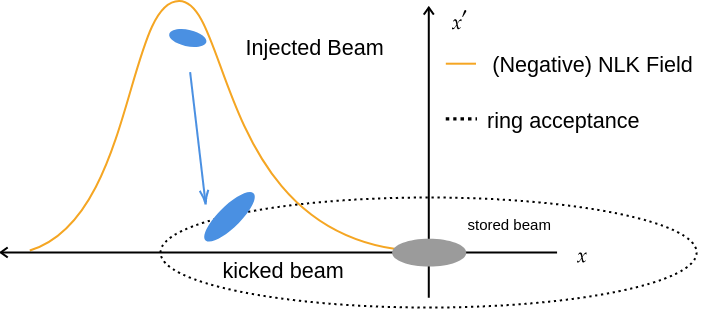
\includegraphics[width=\columnwidth]{Images/inj_cond.png}
    \caption{Injection conditions for DA optimization}
    \label{fig:inj_cond}
\end{figure}

Additionally, one big difference from the early attempt was that families SFP1 and SFB1 were not used as knobs in the optimization experiments since they operate close to their saturation strengthts, where hysteresis effects become significant, as mentioned in section Z. The optimzation experiments were carried out in the machine with the nominal tunes $(\nu_x,\nu_y)=(49.08, 14.14)$, which we shall name Working Point 1 (WP1), as well as in the $(49.20, 14.25)$ and $(49.16, 14.22)$ tunes, Working Points 2 (WP2) and 3 (WP3), respectively. As mentioned before, the motivation was to seek a different optics rendering smaller orbit amplification factors to improve orbit stability.
% The Results reported here have also been presented in Ref.\cite{velloso:ipac23-wepl087} (on WPs 1 and 2) and on the presentation  delivered at the Optics Tuning and Corrections for Future Colliders Workshop.

% The major differences from the previous experiments consisted on
% \begin{itemize}
%     \item the use of the average injection efficiency of 5 injection pulses at $2~\unit{Hz}$ objective function to reduce the experimental noise sigma from $\sigma=\pm8\%$ to $\pm1\%$.
%     \item
%     \item Knobs selection was based in choosing linear combinations spanning null space of the chromaticity response matrix for Working Points 1 and 2. See Ref.~\cite{velloso:ipac23-wepl087} for details. Working Point 3 knobs were chosen as described in section 9.1.
% \end{itemize}
\subsection{Optimization in Working Point 1 (49.08, 14.14)}
The knobs selection scheme was that of the Constrained Scheme I, discussed in section X. Three optimization experiments were carried out. Rendering three optimized configurations found. In Run 1, the optimization was started from the reference sextupole configurations. The machine had its linear optics and orbit corrected, and the optimzation was fired. Upon reaching the best injection efficiency, the run was stopped and the best-perfoming sextupole configurations were saved. The optimum configurations found shall be refered to as "solutions". Magnets were standardized and the run 1 solution was loaded in the machine. Run 2  started from run 1 solution. The horizontal offset was increased even further during the injection to reduce the efficiency and move the beam towards the border of the expectedly increased DA. Run 3 started from the run 2 solution. The figure below shows the objective function history throughout the optimization runs in working point 1.
\missingfigure{optimization history}
\subsubsection{Characterization of solutions}
For each one of the best configurations found during runs 1, 2 and 3 and also for the non-optimized reference configuration (ref. config.), turn-by-turn (TbT) BPM data of the stored beam kicked with the horizontal dipolar kicker was acquired. The DCCT current monitor allowed the determination of the current losses as a function of the horizontal kicks, which is shown in Figure~\ref{fig:loss_kicks}. This curve characterizes the beam's kick resilience.

TbT data also allowed for the reconstruction of the $(x,x^\prime)$ phase space of the beam under the influence of the kicks. Using two BPMs at the ends of an empty ID straight section, the position and angle of the beam were determined at each turn.
Figure~\ref{fig:oldtunes_phase} shows the measured phase spaces for the ref. config. and the best configurations found during run 1, 2, and 3, at the fifth straight section (SA05), which is a high-beta section with identical optics to the injection point. In the measurement, the beam was under the influence of kicks rendering approximately the same current loss of $12\%$.
\begin{figure}[!t]
    \begin{minipage}{0.48\textwidth}
        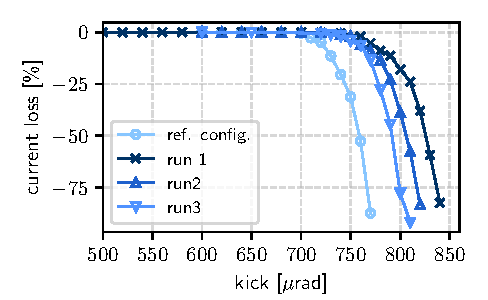
\includegraphics[width=\textwidth]{Images/WEPL087_f1.pdf}
       \caption{Current losses vs. horizontal dipole kick for the ref. config. and for the RCDS solutions at WP 1.}
       \label{fig:loss_kicks}
    \end{minipage}
    \hfill
    \begin{minipage}{0.48\textwidth}
        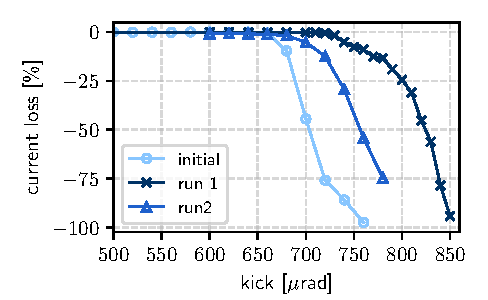
\includegraphics[width=\textwidth]{Images/WEPL087_f3.pdf}
        \caption{Current losses vs. horizontal dipole kick for the initial configuration and the RCDS solutions at WP 2.}
        \label{fig:loss_kicks_newtunes}
    \end{minipage}
\end{figure}

\begin{figure}[!h]
    \begin{minipage}{0.48\textwidth}
        \centering
        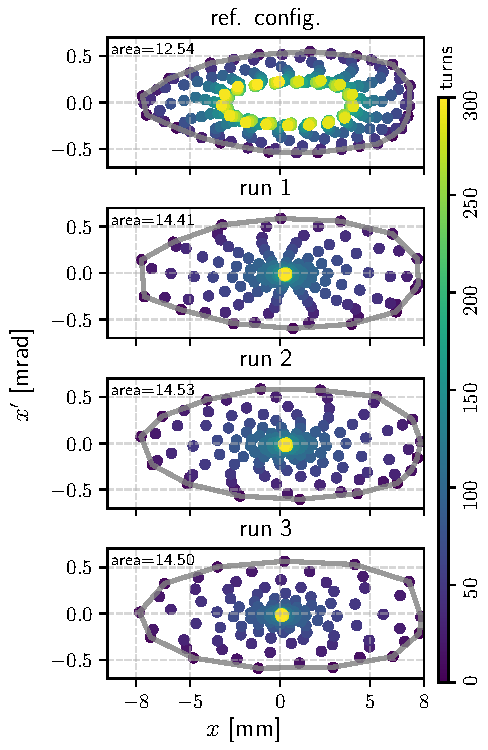
\includegraphics[width=\textwidth]{Images/WEPL087_f2.pdf}
        \caption{Measured phase space at SA05 high-beta straight section for the ref. config. and the best RCDS configurations of runs 1, 2 and 3 in WP 1. Color-map indicates the turns. The areas are in $\unit{mm}~\unit{mrad}$. The beam was being kicked horizontally at $730~\unit{\micro rad}$ in the ref. config, $790~\unit{\micro rad}$ in run 1, $780~\unit{\micro rad}$ in run 2, and $770~\unit{\micro rad}$, in run 3. Loss rates of  $12\%, 11\%, 13\%$ and $13\%$.}
        \label{fig:oldtunes_phase}
    \end{minipage}
    \hfill
    \begin{minipage}{0.48\textwidth}
        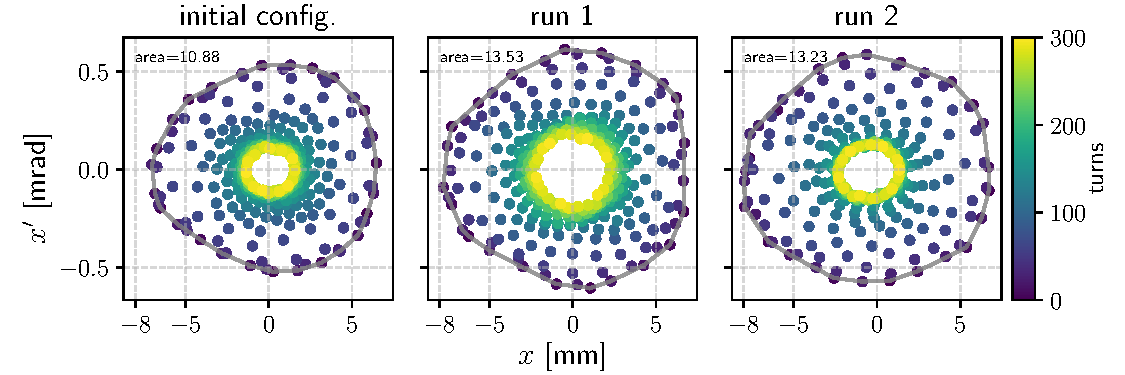
\includegraphics[width=\textwidth]{Images/WEPL087_f4.pdf}
        \caption{Measured phase space at SA05 high-beta straight section for the initial configuration and the best RCDS configurations of runs 1 and 2 in WP 2. Color-map indicates the turns. The areas are in $\unit{mm}~\unit{mrad}$. The beam was being kicked horizontally at $680~\unit{\micro rad}$, for the initial configuration, $770~\unit{\micro rad}$ for run 1, and at $720~\unit{\micro rad}$ for run 2. Loss rates of $10\%$, $12\%$ and $12\%$, respectively}
        \label{fig:newtunes_phase}
    \end{minipage}

\end{figure}
Table~\ref{table1} compiles the injection efficiencies (IE) achieved for each configuration during off-axis NLK injection in normal injection conditions ($x\approx -8.5~\unit{mm}$, $x^\prime\approx 0 $).
Again we stress the apparent elasticness of the phase portrait ellipses deformations: the configuration with the largest kick resilience, that of run 1, is not the one with the largest phase space area and IE performance. This behaviour could be explained if the phase space deformations of the ellipse at the kicker location for this sextupole setting resulted in a larger $x^\prime/x$ ratio, which would account for a larger kick acceptance and the worse injection performance compared to run 2. Summing up, increased kick resilience does not necessarily translates into increased DA.

Lifetime at $60~\unit{mA}$ was measured at $20~\unit{hr}$ for run 2 solution, the best performing in terms of injection efficiency. The measurement revealed no impact of the optimization procedure on liftime, since lifetime for the same conditions on the reference configuration is $21~\unit{hr}$.

Despite the care not to change chromaticity during the procedure with the selection of the chromaticity Jacobian nullspace knobs, a small build-up was observed. Chromaticity was measured as $(2.33, 2.53)$ in ref. config. and $(2.24, 2.39)$ in run 2 solution. This is possibly due to small mismatches between the machine computer model and the real machine, since the optimization knobs computed using the storage ring computer model Jacobian. Despite the small chromaticity changes, the values observed are still acceptable values according to the criteria related to impedances budgets.
\todo[inline]{clarify this}

In summary, for WP1:
\begin{itemize}
    \item the solution found during run 2 rendered $98\%$ injection efficiency,
    \item increase in horizontal phase sapce area and horizontal kick resilience were observed,
    \item no significant effect was observed on beam lifetime,
    \item small, acceptable chromaticity changes observed.
\end{itemize}
The first two items are strong indicators of a DA enlargement.
\begin{table}[]
    \caption{Injection efficiencies (IE) for configurations found for Working Points 1, 2 and 3.}
    \centering
    \begin{tabular}{cccccc}
    \hline
    \multicolumn{2}{c}{working point 1} & \multicolumn{2}{c}{working point 2}         & \multicolumn{2}{c}{working point 3}         \\ \hline
    configuration      & IE $[\%]$      & configuration        & IE $[\%]$            & configuration        & IE $[\%]$            \\ \hline
    ref. config.       & $88\pm8$       & initial              & $51\pm1$             & initial              &                      \\
    run 1              & $91\pm1$       & run 1                & $79\pm3$             & optimized            & $93\pm3$             \\
    run 2              & $98\pm1$       & run 2                & $65\pm1    $         &                      &                      \\
    run 3              & $87\pm3$       & \multicolumn{1}{l}{} & \multicolumn{1}{l}{} & \multicolumn{1}{l}{} & \multicolumn{1}{l}{} \\ \hline
    \end{tabular}
    \label{table1}
    \end{table}


\subsection{Optimization in Working Point 2 (49.20, 14.25)}
The storage ring tunes were adjusted to $(\nu_x, \nu_y)=(49.20, 14.25)$ using the tune quadrupole knobs, as discussed in section X. The sextupole configuration was the same as the nominal tunes reference configuration. The new optics significantly impacted on the DA, since the injection efficiency in nominal conditions with this setup was about $50\%$, at most. Without succesful optimization, it would be impossible to operate in this working point.

For the optimzation experiment, the objective function was the injection efficiency with the the beam delivered at the upper-left border of the $x,x^\prime$ phase-spacek, just as in the WP2 experiment. The optimization knobs were those of the Constraints Scheme II, discussed in Y, totalling 17 independent knobs. In working point 2, two optimization runs were carried out: run 1 and run 2. The sextupoles were optimized from the new tunes optics with reference sextupoles and then, from the best solution found in run 1, run 2 was launched. The objective function history throughout the optimzation is shown in Figure
\missingfigure{obj func history}
\subsubsection{Characterization of solutions}
Injection efficiency in nominal conditions is highlighted in Table~\ref{table1}. Despite observing improvements, the best performing configuration, the solution found in run 1, still provides an unsatisfactory efficiency for operation.

TbT BPM data of the kicked stored beam  in the initial configuration (non-optimzed) and in each run's best solution was acquired and allowed the determination of current losses vs. kicks, shown in Fig.~\ref{fig:loss_kicks_newtunes}, and the reconstruction of phase space, shown in Fig. ~\ref{fig:newtunes_phase}. Improvements on the resilience and the phase-space area can be observed.

The configuration found during run 1 rendered the best injection efficiency, the largest kick resilience. It also displayed larger lifetime than the initial configuration ($21~\unit{hrs}$, run 1 vs. $18~\unit{hrs}$, initial, at $60~\unit{mA}$) which is comparable to the reference configuration lifieme. The largest phase-space area increase was also observed for this solution. Still, the injection efficiency delivered by the best performing solution on this working point was quite unsatisfactory and optimizing in this working point was hard, as the objective function history shows. The DA seemed more rigid. For these reasons, another working pouint was sought. If the idea is to increase the fraction parts of the tunes, and $(0.20, 0.25)$ seemed like overshooting, optimzation in the intermediate tunes between WP1 and WP2, with fractional tunes $(0.16, 0.22)$, seemed reasonable.
\subsection{Optimization in Working Point 3 (49.16, 14.22)}
From the reference configuration with corrected linear optics and orbit, the tunes were adjusted to the desired working point $(\nu_x, \nu_y)=(49.16, 13.22)$. The injection efficiency was again lower, indicating, as in WP2, deterioration of the DA.

The objective function was injection efficiency in the same conditions as in WP1 and WP2 experiments. The optimzation knobs were those of the Compensation Scheme described in section X. The search space was 13-dimensional. Two optimization runs were carried out, starting from sextupole settings of the reference configuration. Best configuration found at run 1 was reloaded after magnets standardization and run 2 was launched. Only run 2 configuration was saved. The figure shows the objective function history.
\missingfigure{obj func hist}
\subsubsection{Characterization of the solution}
The optimized solution was characterized in terms of kick resilience, phase space area, injection efficiency and whether it preserved chromaticity and lifetime.  Lifetime at $60~\unit{mA}$ was measured at $19.5~\unit{hrs}$, so no significant reductions were observed. No significant chromaticity changes were observed as well. Phase space area increased, compared to the initial non-optimized configuration, and it reached similar area to that of the nominal tunes reference configuration, as Figure shows. Kick resilience, shown in Figure, also improved, with a larger fraction of the beam surviving to large kicks in the range from $700-770~\unit{\mu rad}$. Most importantly, run 2 solution displayed injection efficiency of $93\pm3\%$ during nominal off-axis injection, which is acceptable for operation.
\begin{figure}[htb]
    \begin{minipage}{0.48\textwidth}
        \centering
        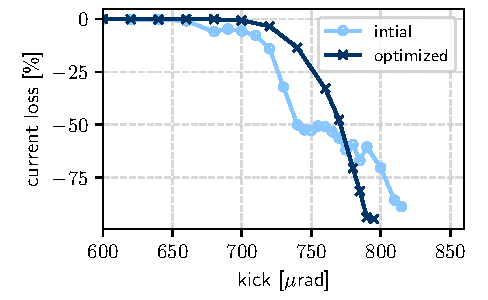
\includegraphics[width=\textwidth]{Images/wp3_kick_resilience.pdf}
        \caption{Current losses vs. horizontal dipole kick for the initial configuration and the RCDS solution at WP 3}
    \end{minipage}\
    \hfill
    \begin{minipage}{0.48\textwidth}
        \centering
        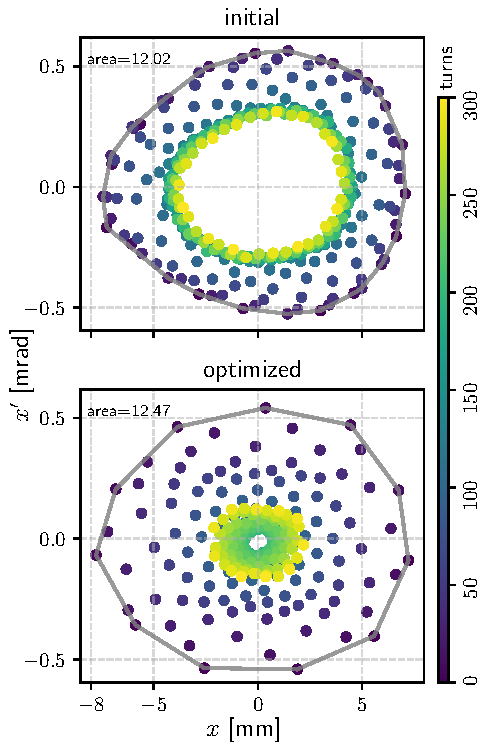
\includegraphics[width=\textwidth]{Images/wp3_phase_space.pdf}
        \caption{Measured phase space at SA05 high-beta straight section for the non-optimized configuration and the best RCDS configuration in WP 3. Color-map indicates the turns. The areas are in $\unit{mm}~\unit{mrad}$.}
    \end{minipage}
\end{figure}
\subsubsection{Orbit Stability}
Orbit stability improvements were confirmed by the orbit integrated spectrum density, which decreased by a factor of approximately 2 \cite{Liu:IPAC23-WEOGA2}. Orbit rms variations reached the record values of less than $1\%$ of the horizontal beam size, in the horizontal plane, and less than $4\%$ of the vertical beam size in the vertical plane.

% In summary, in the experiments throughout 2023, the noise in the objective function was reduced and the injection efficiency average was established as the standard objective. No significant chromaticity changes were observed during/after the optimization runs, nor significant changes to beam lifetime, compared to the nominal working point reference configuration.

% Excellent configurations were found in WP1, with 98\% injection efficiency, but we still believe there is room for further improvements in the higher tunes configurations.
\begin{figure}[htb]
    \centering
    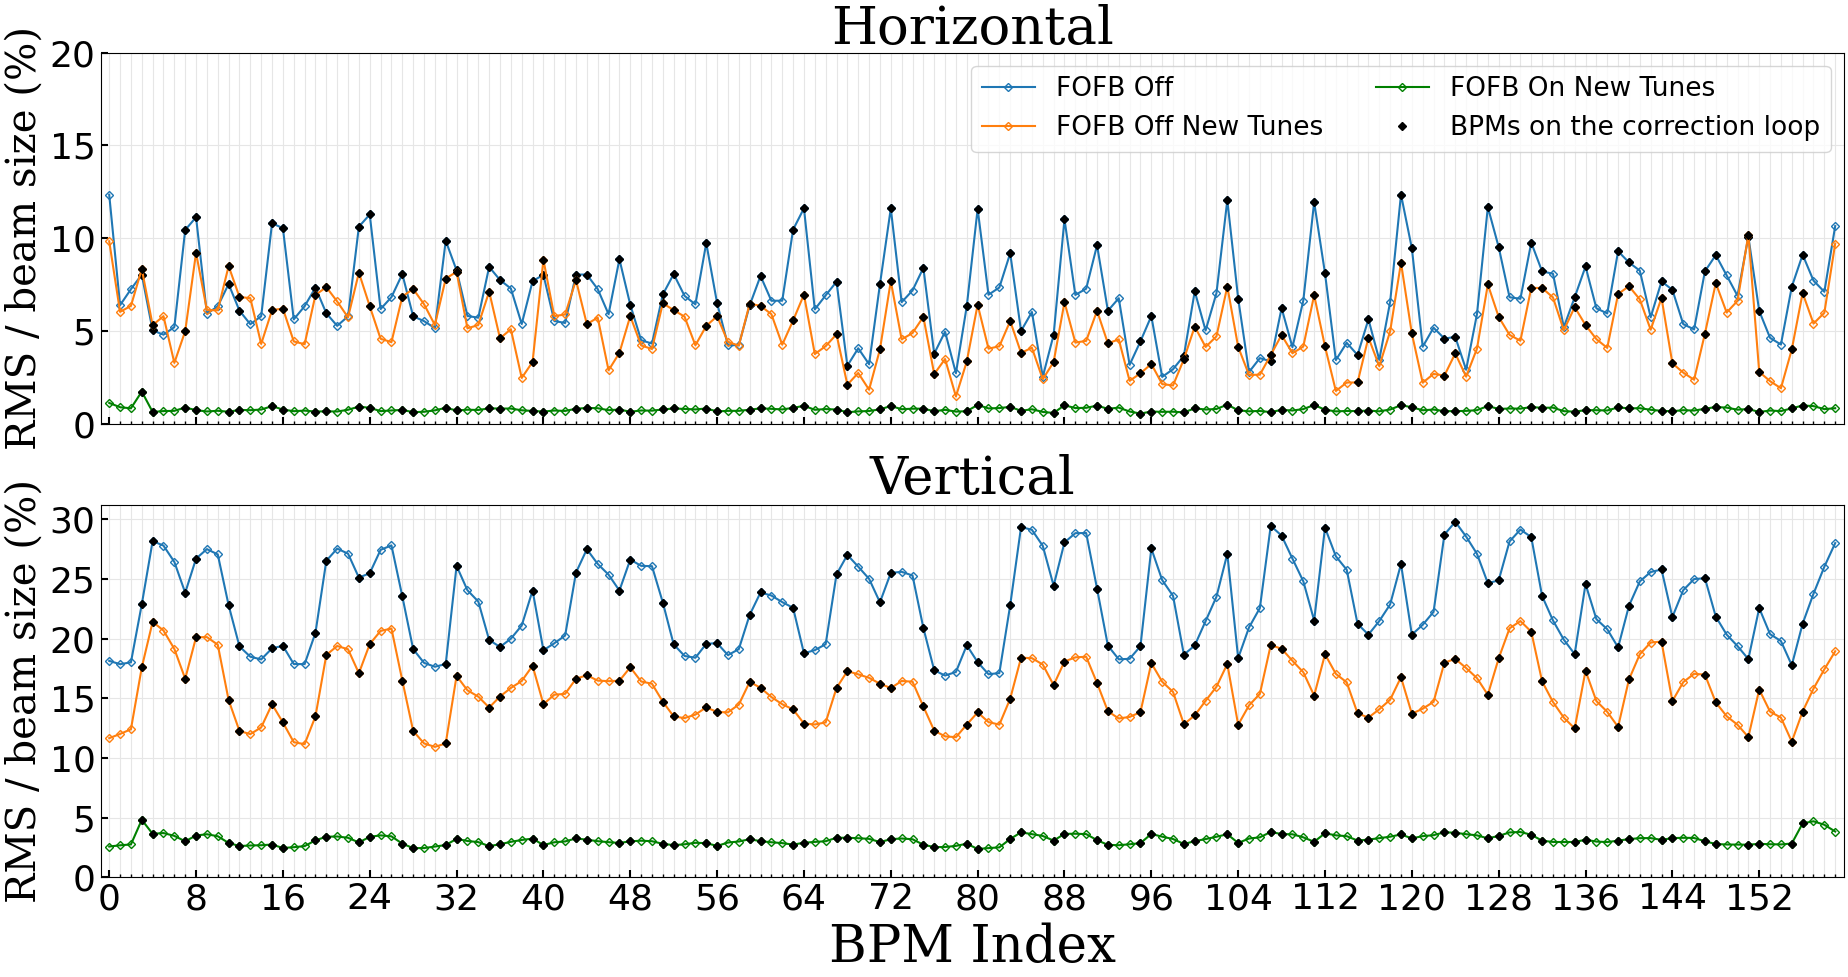
\includegraphics[width=\textwidth]{Images/WEOGA2_f5.png}
    \caption{Horizontal/Vertical RMS orbit variations in units of the horizontal and vertical beam sizes. Blue curves represents variations in the nominal working point, WP1, orange curves are the orbit variations at WP3, and green curves variations at WP3 plus results of the recent improvements in Fast Orbit Feedback System. From~\cite{Liu:IPAC23-WEOGA2}}
\end{figure}
% \section{Sobre o Estudante e Perspectivas}
% O estudante é bacharel em Física pelo Departamento de Física da Universidade Federal de São Carlos (DF-UFSCar), graduado em 2021 com e média geral de $9.3/10$. Durante a graduação participou de atividades de ensino, divulgação e pesquisa, dentre as quais destacam-se: atuação como professor e monitor no Cursinho Pré-Vestibular Comunitário da UFSCar; participação do comitê de organização da Semana da Física da UFSCar de 2018; realização projetos de Iniciação Científica em Relatividade Geral\footnote{Processo FAPESP \href{https://bv.fapesp.br/pt/bolsas/184970/introducao-a-relatividade-geral-e-aplicacoes/}{19/03968-2}} e em Teoria Quântica de Campos\footnote{Processo FAPESP \href{https://bv.fapesp.br/pt/bolsas/192776/introducao-a-teoria-quantica-de-campos/}{ 20/06955-6}}; estágio junto ao Grupo de Física de Aceleradores do Laboratório Nacional de Luz Síncrotron; Trabalho de Conclusão de Curso versando sobre ``Amplitude de Propagação para a Partícula Relativística e uma Introdução à Teoria Quântica de Campos"\ aprovado com nota máxima; além da participação de diversas escolas de verão, \textit{workshops} e seminários, em especial a \textit{Modern Physics at all Scales Summer School}, realizada pela Universidade de Leiden, em Leiden, Países Baixos, para a qual o estudante foi selecionado para participar com auxílio financeiro total.

% O trabalho \textit{Orbit Response Matrix Measurement via Alternating Excitation of Orbit Correctors at SIRIUS} realizado durante o estágio junto à FAC consistiu na implementação de um método rápido para medida de matriz resposta de órbita do SIRIUS e está sendo preparado para submissão nos \textit{proceedings} da \href{https://www.ipac22.org/}{\textit{13th International Particle Accelerator Conference}}.

% Recém ingresso ao curso de mestrado em Física, o estudante está inscrito nas disciplinas ``FI001 - Mecânica Quântica I" e ``FI004 - Física Estatística I", e tem perspectivas ainda de cursar ``FI195 - Mecânica Avançada", ``FI008 Eletrodinâmica I" (diretamente relacionadas com a dinâmica de feixe em aceleradores) e outras necessárias para a integralização de créditos.

% \section{Conclusions}
% The MSc. project is being developed on shcedule and should be completed within the stipulated duration of the grant. In the reported period from August 2022 to July 2023 the student has completed the graduate program requierements for course credits, co-athoured and collaborated in the writing of computer code for performing machine experiments, participated in the experiments and performed all the analysis of the obtained data. The student has also co-authored and submitted contributions to IPAC'23, the largest conference in the field of particle accelerators, and presented the results achieved so far during the project in the Optics Tuning and Corrections for Future Colliders Workshop, at CERN.

% The work developed alongside the LNLS Accelerator Physics Group has contributed to the recent achievements of record orbit stability at the SIRIUS storage ring.

% More experiments for further optimzation, exploration of working points and and characterizations of nonlinear dynamics performance should proceed in the upcoming months up until the end of the year, when the student should then focus in the writing of his dissertation.\
\section{Amplitude-dependent tune-shift analysis}
